\chapter{\noun{Current Situation}   }

The main element of the currently used system is a paper prescription. There are all the informations, which allow a patient to buy specific medicines, e.g.: 

\begin{itemize}
  \item prescription’s creation date,
  \item patient’s personal data:
  \begin{itemize}
	  \item name and surname
	  \item address
	  \item PESEL
  \end{itemize}
  \item number of the prescription, specific for each doctor \footnote{NFZ generates a list of prescription for each doctor. Every prescription has the unique identifier number. During the refoundation process, NFZ checks, if the number on the prescription, the doctor name, signature and stamp are correct. Only if thy are valid, the refoundation is granted.  },
  \item list of medicines with refoundation level,
  \item signature and stamp of the doctor. 
\end{itemize}

The patient, who was given the prescription by the doctor, goes to the pharmacy to buy the medicines. He gives his prescription to a pharmacist and says which of the medicines from the list he wants to buy. The pharmacist checks if the medicines are available and if yes, he sells them. Next, he takes the prescription and makes a signature next to the each of the medicine he sold. He also inputs to the software installed on computers in the pharmacy, which of the medicine was sold, for who, who gave the prescription and what are the refoundation costs.

Each month in every pharmacy a report, consisting of  the set of the information about each prescription sold in the pharmacy is generated. This report is sent to the NFZ central database. Based on this, the NFZ refunds costs of the medicines. Each prescription has to be kept for at least five years in the pharmacy, and be ready for checking during controls made by NFZ representatives. 

\begin{figure}	
	\hspace*{0.8in}
    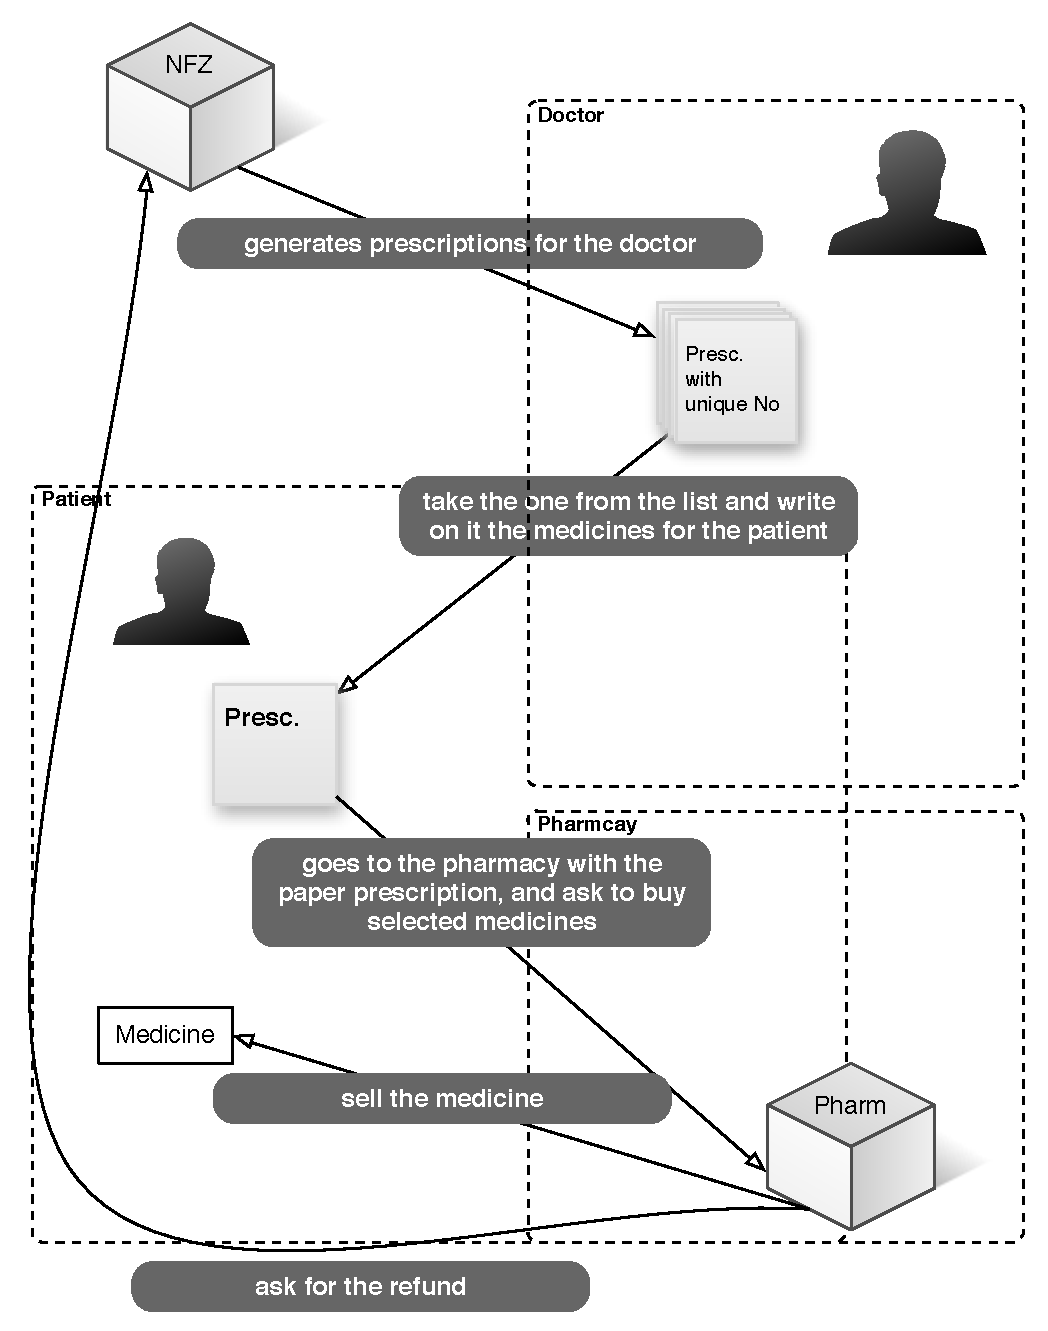
\includegraphics[scale=0.6]{cs.pdf}
    \caption{The main points of currently used system}
    \label{fig:mp_cs}
\end{figure} 